\section{Quadratic}
\label{sec.quadratic}


We have the plots of two quadratic polynomials shown in Figure~\ref{fig.parabola}.
Each plot takes the geometric form of a parabola.  As can be seen in the figure,
the parabola might intersect the x-axis twice [Left], once [Center], or not at all [Right].

\begin{align*}
  P_1(x) &= 2x^2 - 2 x - 5\\
  P_2(x) &= x^2 -x + \frac{1}{4}\\
  P_3(x) &=  -2x^2 + 2x -2
\end{align*}

%% derived from https://tex.stackexchange.com/questions/357538/graph-of-a-parabola-on-pgfplots
%% Thanks to Stefan Pinnow
%%     https://tex.stackexchange.com/users/95441/stefan-pinnow

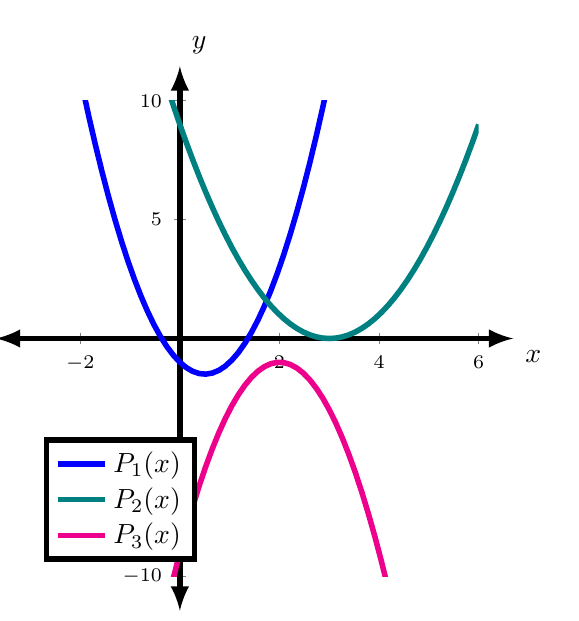
\begin{tikzpicture}
  \begin{axis}[
      legend pos=south west,
      width=.6\textwidth,
      height=3in,
      axis lines=middle,
      xmin=-3,
      xmax=6,
      ymin=-10,
      ymax=10,
      scaled ticks=false,
      line width=2pt,
      ticklabel style={font=\scriptsize},
      xlabel=$x$,
      ylabel=$y$,
      samples=70,
      domain=-3:6,
      axis line style={
        latex-latex,
        shorten >=-12.5pt,
        shorten <=-12.5pt,
      },
      xlabel style={at={(ticklabel* cs:1)}, xshift=12.5pt, anchor=north west},
      ylabel style={at={(ticklabel* cs:1)}, yshift=12.5pt, anchor=south west},
    ]
    
    \addplot[color=blue] {2*x^2 - 2*x - 1}; % 2 roots
    \addlegendentry{\(P_1(x)\)}
    \addplot[color=teal] {x^2 - 6*x + 9}; % 1 root
    \addlegendentry{\(P_2(x)\)}
    \addplot[color=magenta] {-2*x^2 + 8*x - 9}; % 0 roots
    \addlegendentry{\(P_3(x)\)}
  \end{axis}
\end{tikzpicture}
%


In the case of $P_1$, the two x-intercepts can be found using the quadratic formula, using $a=2$, $b=-2$, and $c=-5$

\begin{align*}
  x &= \frac{-b~ \pm \sqrt{b^2 - 4a c}}{2a}\\
  &= \frac{-(-2)~ \pm \sqrt{(-2)^2 - 4 (2) (-5)}}{(2)(2)}\\
  &= \frac{2 ~\pm \sqrt{4 + 40}}{4}
  = \frac{1}{2} \pm \frac{1}{2}\sqrt{11}
\end{align*}

In the case of $P_2$, we do the same, but with $a=1$, $b=-1$, and
$c=\frac{1}{4}$, where we find the discriminant $b^2 - 4a c = 1^2 -
(4)(1)(\frac{1}{4}) = 1 - 1 = 0$.  Thus there is exactly one root.
The existance of a single root can be seen in
Figure~\ref{fig.parabola}~[Center] by the fact that the parobala
touches the x-axis tangentially.

Finally, In the case of $P_3$, if we attempty the same, but with $a=-2$, $b=2$, and $c=-2$, we see
that the discriminant is $b^2 - 4a c = (-2)^2 - (4)(-2)(-2) = 4 - 16 = -12 < 0$.  When the discriminant
is negative, there are no \emph{real} roots.  This can be seen in
Figure~\ref{fig.parabola}~[Right] by the fact that the parobola does not
touch the x-axis at all.

\begin{listing}{Function to compute roots of a quadratic polynomial.}{code.quadratic}
\begin{minipage}[c]{0.95\textwidth}\begin{lstlisting}
def find_quadratic_roots(a, b, c):
    epsilon = 0.001
    discriminant = b * b - 4 * a * c
    if a == 0 :
        return find_x_intercept(b,c)
    if discriminant > epsilon:
        return sorted([(-b + sqrt(discriminant)) / (2 * a),
                       (-b - sqrt(discriminant)) / (2 * a)])
    elif abs(discriminant) < epsilon:
        return [-b / (2 * a), 
                -b / (2 * a)]
    else:
        return []
\end{lstlisting}\end{minipage}\end{listing}

